\chapter{Diffusive model application on wire compensators losses}\label{ch:wire-compensators}

In this chapter, we examin the case of beam-beam wire compensators, which play an important role in counteracting the detrimental effects of beam-beam interactions in the LHC. Our original contribution to this field is the application of our diffusive model to assess the long-term effects of wire compensators on beam losses and emittance.

Through the study of the LHC Beam~2 data, collected during a Run~2 measurement campaign, we aim to understand the effectiveness of wire compensators in mitigating beam-beam effects without causing unwanted effects such as increased emittance. The results of this analysis provide insight into the potential benefits of utilising wire compensators in present and future accelerator design and show how this diffusive model can be applied to assess long-term effects of new components in the accelerator via inspection of the beam loss data.

The chapter is structured as follows. In Section~\ref{sec:5:wire-compensators}, we present the generalities of wire compensators and their implementation in the LHC. In Section~\ref{sec:5:wire-data}, we give an overview of the data gathered during the dedicated wire compensators' measurement campaign in Run~2. In Section~\ref{sec:5:wire-model}, we discuss how our diffusive model can be applied to the data and, in Section~\ref{sec:5:results}, we present the results of the analysis. Finally, in Section~\ref{sec:5:conclusions}, we draw our conclusions and discuss the potential future applications of the diffusive model in light of the results and difficulties encountered in this analysis.

\section{Generalities on LHC beam-beam wire compensators}\label{sec:5:wire-compensators}

One of the most significant limits in the present LHC design and the future HL-LHC is given by the electromagnetic interactions between the two counter-rotating beams in the shared sections of the machine that occur around the interaction points~\cite{Arduini_2016}. These beam-beam interactions lead to what can be distinguished as head-on beam-beam effects, which occur when the beam bunches overlap at the interaction point, and long-range beam-beam effects, occurring when the two beams are transversely separated in the remaining part of the shared region.

In the LHC, the beams are set in collision with a \textit{crossing angle}, which has the purpose of separating bunches immediately upstream and downstream of the collision point~\cite{Arduini_2016} to reduce the strength of long-range beam-beam effects. However, an increase in the crossing angle also implies a reduction in integrated luminosity, that is, the total number of collisions that have occurred over a given period of time, typically measured in inverse femtobarns \SI{}{fb}$^{-1}$~\cite{Herr:941318}, as the overlap of the bunches decreases. A schematic visualisation of two different crossing angles and their consequent effect on beam separation and bunch overlap is presented in Fig.~\ref{fig:crossing-angles}. The nominal full crossing angle for LHC is set at $\theta_c =$ \SI{285}{\micro\radian}, while for HL-LHC the expected baseline parameter will be set at $\theta_c =$ \SI{500}{\micro\radian}~\cite{BejarAlonso:2749422}. 

\begin{figure}[hpt]
    \centering
    \def\svgwidth{1.0\textwidth}
    \import{5_wire_compensators_LHC/figs/}{crossing_angle_basics.pdf_tex}
    \caption{Schematic visualisation of two different crossing angles and their consequent effect on beam separation and bunch overlap. As $\theta_{c1} > \theta_{c2}$, the bunches are more separated in the first case (left), while the bunch overlap is larger in the second case (right). The long-range beam-beam effects are also more significant in the second case.}
    \label{fig:crossing-angles}
\end{figure}

To address long-range beam-beam effects while maintaining a small crossing angle, a corrective approach based on electromagnet lenses was presented in~\cite{Koutchouk:692058}. The core concept of this approach is to compensate for the perturbation pattern given by long-range effects by using DC wires. The idea of using DC wires comes specifically from the observation that these long-range effects are similar to the $1/r$ dependence similar to the electric field potential generated by a simple wire~\cite{PhysRevSTAB.5.074001}. A sketch of the concept of compensation given by the BBCW is presented in Fig.~\ref{fig:wire-baseline}.

\begin{figure}[hpt]
    \centering
    \def\svgwidth{1.0\textwidth}
    \import{5_wire_compensators_LHC/figs/}{crossing_angle_kick.pdf_tex}
    \caption{Left, sketch of the long-range beam-beam effects experienced by Beam~2 from Beam~1, following the weak-strong approximation (i.e.\ we consider the effect of Beam~1 on Beam~2 and not vice versa). Right, sketch of the principle of the compensation given by the BBCW. The long-range beam-beam effects (red arrow) are compensated by the DC wires (green arrow), which are placed in the beam path before and after the interaction point.}
    \label{fig:wire-baseline}
\end{figure}

The resulting tool is called \textit{``beam-beam wire compensator''} (BBCW), and it has been tested in multiple iterations on various accelerator complexes (a complete list of experimental applications up to early 2022 is available in~\cite{axel.wires}).

In the LHC, the BBCW are installed for Beam~2 only, as it was the only beam that was expected to operate with a coronograph~\cite{Goldblatt:2313940}, which is a device that is expected to allow transverse beam halo measurements in the future. The wires are embedded in the tertiary collimators placed upstream and downstream of IP1 and IP5~\cite{Rossi:2696270}. These collimators are still part of the collimator hierarchy, presented in Section~\ref{sec:4:collimation}, and are placed near the IPs to locally protect the experiments from potentially damaging losses.

A collimator hosts two separate wires (one per jaw), and each wire can carry up to \SI{350}{\ampere}. These two separate wires are cabled in series so that they have the same polarity. This configuration enables a specific 2-jaw powering setup with the characteristics of doubling the odd multipolar strength of the kick, while the even ones cancel out. This choice is motivated by the need to compensate for octupolar resonances~\cite{Poyet:2703503}. The two possible configurations are presented in Fig.~\ref{fig:wire-configs}. The first, called the \textit{single wire} configuration, powers only the internal wires. The second one, called \textit{quadrupolar configuration}, powers both wires.

\begin{figure}[hpt]
    \centering
    \def\svgwidth{1.0\textwidth}
    \import{5_wire_compensators_LHC/figs/}{crossing_angle_configs.pdf_tex}
    \caption{Left, sketch of the single wire configuration, where only one wire per pair is powered. Right, quadrupolar configuration, where both wires in each pair are powered to compensate the octupolar resonances.}
    \label{fig:wire-configs}
\end{figure}

\section{Overview of experimental data}\label{sec:5:wire-data}

For the application of our diffusive framework, we consider the experimental data gathered at the CERN LHC during the 2018 LHC Machine Development (MD) programme, during the BBCW measurements campaign~\cite{Poyet:2703503}. More specifically, we consider the data gathered during fill 7386, as it has the configuration closest to an operational scenario.

During this MD measurement, the BBCW prototypes installed for Beam~2 were tested in various long-range beam-beam-dominated scenarios. During fill 7386, three trains of symmetric bunches were tested at flat-top energy with collisions at different crossing angles, smaller than the nominal one to enhance long-range beam-beam effects. During this operational-like fill, the wire compensators were set in the quadrupolar configuration. The loss signals measured by the BLMs for the two beams are shown in Fig.~\ref{fig:wire-data}, note that the measurement unit is in \SI{}{protons \per s}, as we are considering calibrated losses. In addition to the BLM data, the beam intensity measured by the DCBCTs, the current in the wire, the octupole powering, and the crossing angles are also reported. 

\begin{figure}[hpt]
    \centering
    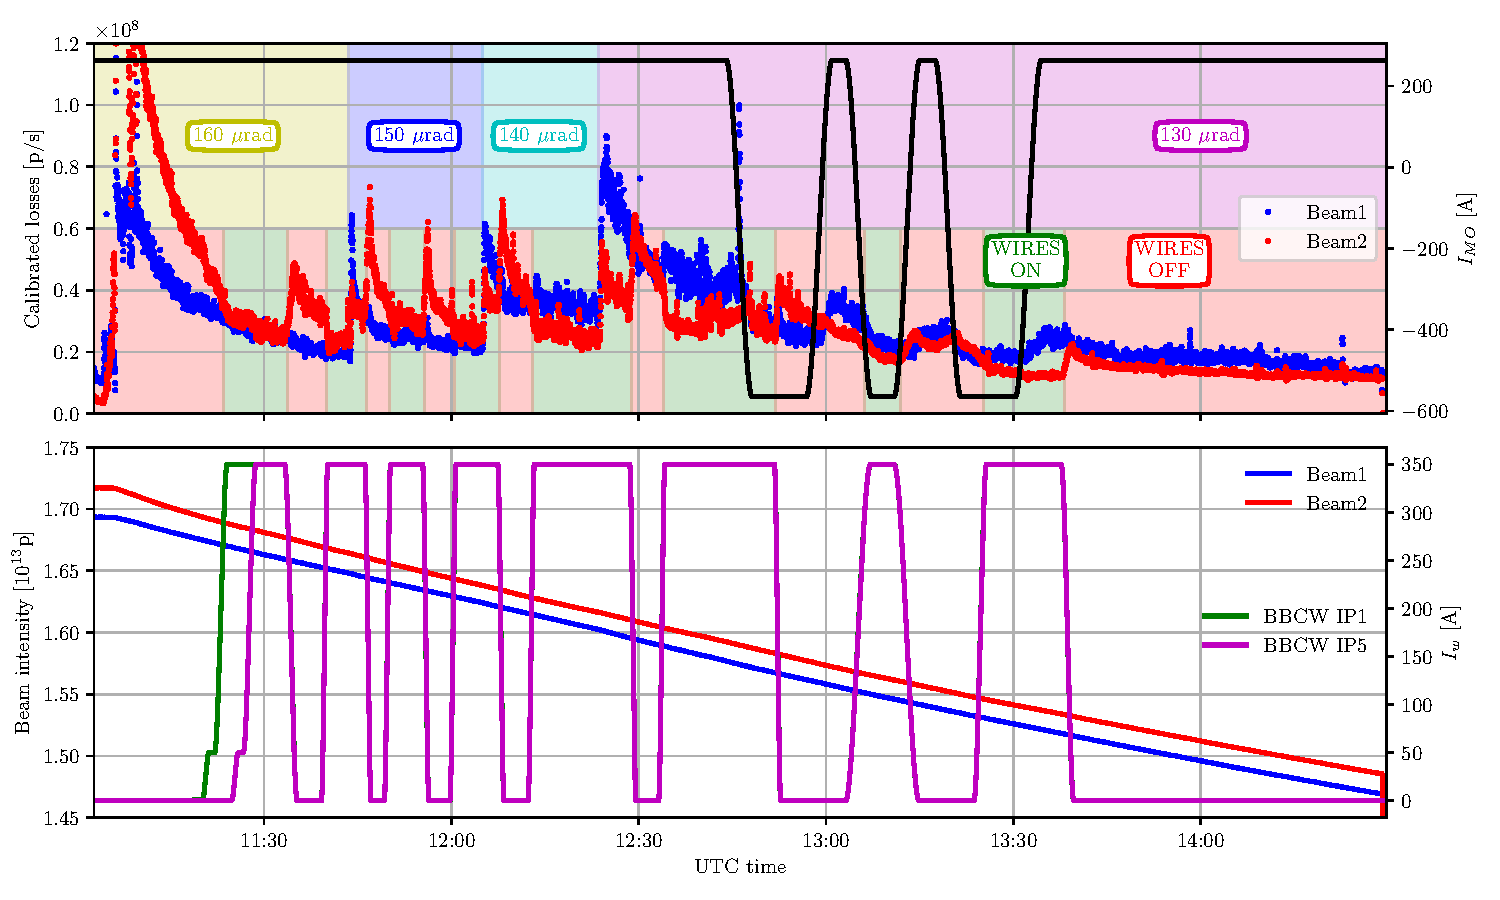
\includegraphics[width=1.0\textwidth]{5_wire_compensators_LHC/figs/wire_summary.pdf}
    \caption{Overview of the data gathered during fill 7386. BLM calibrated losses and BCT beam intensity measurements were taken at different combinations of crossing angles, wire power, and octupole power.}
    \label{fig:wire-data}
\end{figure}

The BLM data for Beam~1 and Beam~2 in units of \SI{}{protons \per s} represents a high-precision measure of protons lost over time. Instead, the DCBCT data provide a measurement of the intensity of the beam in number of protons over time. This measurement is not sensitive enough; it can be seen from the plot how the measured intensity does not distinguish the different regimes of losses highlighted by the BLM data and maintains a steady linear decrease. This difference in sensitivity makes the BLM data a fundamental tool for inspecting the different regimes of losses in the transverse plane.  

BBCW and octupole magnets powering are reported in Ampere. BBCW wires can be found in either an \textit{off} state, namely at \SI{0}{\ampere}, or in an \textit{on} state, namely at \SI{350}{\ampere}. Instead, the octupoles are found at two different current values, namely \SI{260}{\ampere} and \SI{-560}{\ampere}. It is important to highlight how the switch of state for both systems requires a non-negligible amount of time; this will be thoroughly discussed in the next section.

It is possible to see how the data provide a variety of crossing angle configurations, along with on-off alternations of both BBCW power and octupoles current. Qualitatively, one can see how the BBCW equipped in Beam~2 do lead to a lower BLM loss signal when they are turned on, while turning them off leads to a strong peak in the losses measured by the BLMs.

We will now discuss how our diffusive framework can be applied to this loss signal, along with some necessary considerations on how one must preprocess and interpret these data before applying the model. 

\section{Application of the diffusive model}\label{sec:5:wire-model}

Let us consider the Fokker-Planck equation presented in Eq.~\eqref{eq:fp}, with the Nekhoroshev-like form of the diffusion coefficient. We recall that the system is fully characterised by the three free parameters $\epsilon$, $I_\ast$, and $\kappa$.

To apply this model to the BLM data and reconstruct $D(I)$ for the various states of the system, we perform a fitting approach inspired by the procedure used in the work of Bazzani et al.~\cite{bazzani2020diffusion}, where the same Fokker-Planck model is used to reconstruct the evolution of the normalised beam intensity.

Starting from the BLM and DCBCT data collected, we want to construct a measure of the normalised intensity of the beam as a function of the number of turns. We first convert the measurements from seconds to the number of turns, considering that in LHC Run2, a reference proton at \SI{6.5}{TeV} performs 11245 turns every second. We then evaluate the relative intensity lost over an interval $[N_0, N_1]$, as the BCT data are not sensitive enough to measure the small differences in loss rates, we consider the amount of protons lost from the integrated BLM signal, and we take the BCT value registered at the beginning of the interval considered as the reference intensity, as it is the moment at which the first peak in BLM losses was measured. This procedure is illustrated in Fig.~\ref{fig:blm-to-intensity}.

\begin{figure}[hpt]
    \centering
    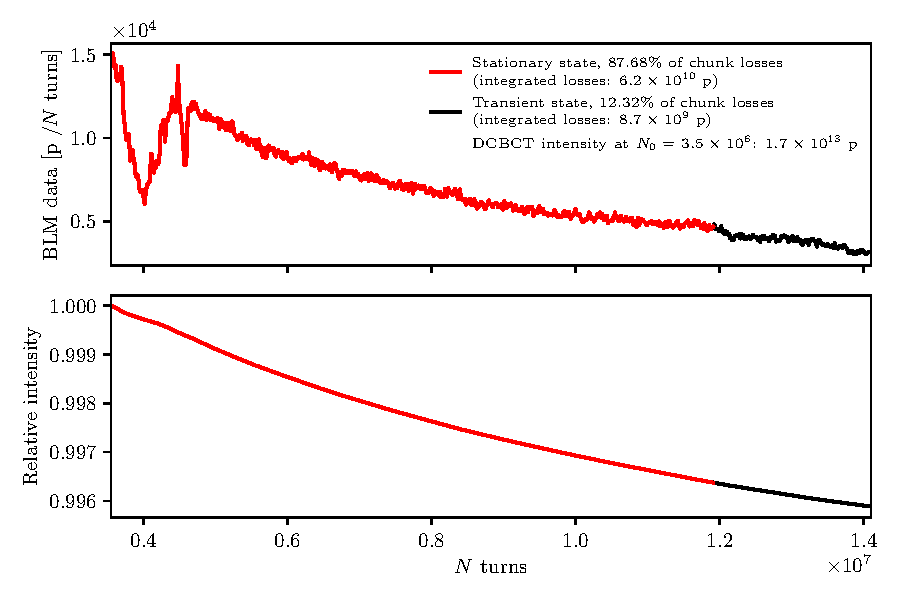
\includegraphics[width=1.0\textwidth]{5_wire_compensators_LHC/figs/stationary_transient_example_chunk.pdf}
    \caption{Example of the procedure used to evaluate the relative intensity lost over an interval $[N_0, N_1]$. The BLM signal is integrated over the interval, and the BCT value registered at $N_0=3.5\times10^6$ turns is used as the reference intensity. A comparison between the integrated losses measured in the stationary state of the chunk and the transient state is also reported. As the losses in the transient state are much lower than the losses in the stationary state, our working hypothesis still holds.}
    \label{fig:blm-to-intensity}
\end{figure}

In addition to the various assumptions made to allow the application of the special form of the diffusion coefficient, it is important to note that this model has the strong assumption that $D(I)$ does not evolve over time. This implies that the magnetic lattice of the accelerator must not manifest stronger variations than those given by the small stochastic perturbation. Such an assumption requires some preliminary consideration on the BLM loss signal that we have at hand.

When the BBCW, the crossing angle, and the octupoles are in a stationary state, we can state that the parameters of the Fokker-Planck equation can be considered as constant over time. We can define this state as stationary and have the beam distribution $\rho(I, t)$ following the evolution defined by the Fokker-Planck equation.

When, instead, a variation in any of the accelerator elements occurs, e.g.\ a BBCW is switched on or the crossing angle is varied, the parameters of the Fokker-Planck equation vary as well into a new value. This variation does not necessarily occur in a negligible time. As can be seen in Fig.~\ref{fig:transient-state}. In fact, switching the BBCW DC current to the target voltage takes a significant number of seconds, leading to a time interval in which the system is in a transient state. During such a transient state, we cannot make assumptions about the evolution of the transverse beam or the evolution of the values of $\epsilon$, $I_\ast$, and $\kappa$, and therefore we are forced to discard these data slices.

\begin{figure}[hpt]
    \centering
    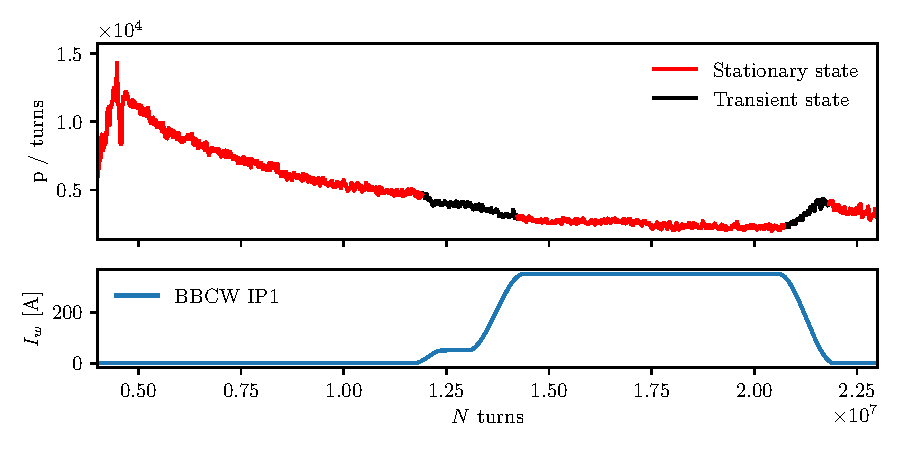
\includegraphics[width=1.0\textwidth]{5_wire_compensators_LHC/figs/stationary_transient.pdf}
    \caption{Visualization of the difference between stationary state and transient state for a data slice. We define as stationary state the time interval in which all the parameters of the system are in a steady state, while the transient state is the time interval in which the system is undergoing a variation. Here, the BBCW DC current is switched on to the target value, causing a transient state along the process.}
    \label{fig:transient-state}
\end{figure}

In Fig.~\ref{fig:chunks}, we show the BLM data for Beam~2 divided into enumerated chunks where the system is in stationary state. We can see how the stationary states are generally longer than the transient states, except for the part where the octupoles change powering.

\begin{figure}[hpt]
    \centering
    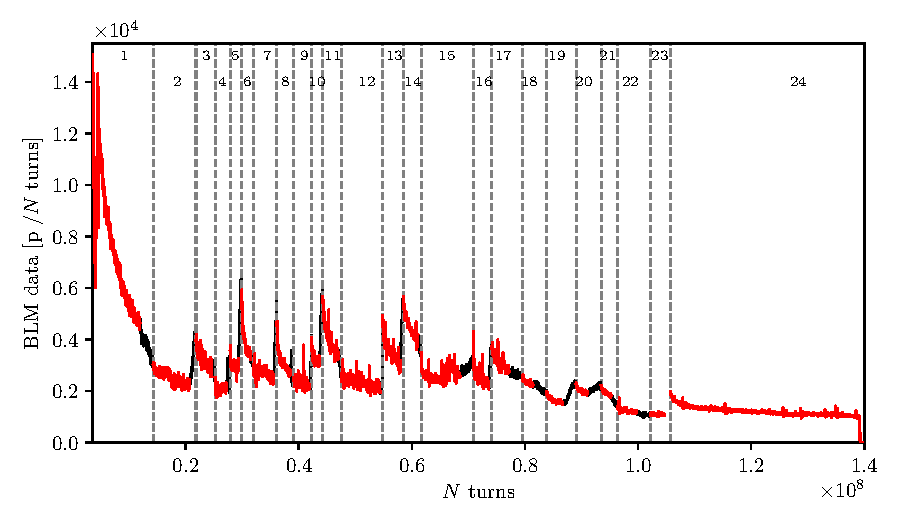
\includegraphics[width=1.0\textwidth]{5_wire_compensators_LHC/figs/chunks_names.pdf}
    \caption{Experimental data for Beam~2 divided in chunks, where each chunk is in a stationary state. Each chunk is characterized by a different set of parameters, and the system is in a transient state when the parameters are changed. Each chunk has a number assigned, which will be used to identify it for the rest of the analysis. Red corresponds to stationary state data, while black represents transient state data.}
    \label{fig:chunks}
\end{figure}

We assume that the beam distribution at the end of a stationary state can be used as the initial condition of the next stationary state. Therefore, we completely neglect the transient state losses between the two stationary states. However, to justify this approach, we must verify that the integrated loss in the transient state is significantly smaller than the integrated loss in the stationary state.

In Fig.~\ref{fig:wire_loss_comp}, this comparison is shown for each individual chunk, and it is possible to see how the interval where the octupole state changes has higher relative transient losses. Such comparable losses led us to the decision not to inspect this chunk of data characterised by varying octupoles, and we performed our fitting procedure only to the data up to those variations.

\begin{figure}[hpt]
    \centering
    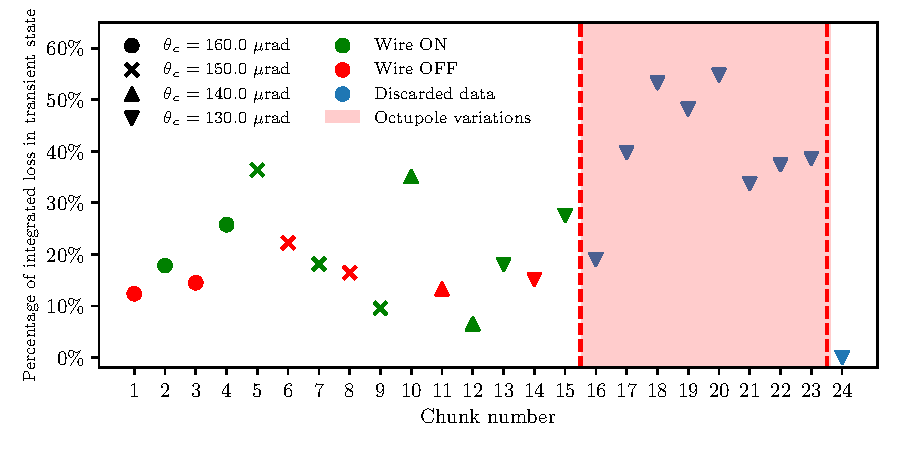
\includegraphics[width=1.0\textwidth]{5_wire_compensators_LHC/figs/losses_comparison.pdf}
    \caption{Comparison of the integrated losses in transient state and in stationary state for each chunk of data. The chunk number follows the nomenclature defined in Fig.~\ref{fig:chunks}. A higher relative loss in the transient states can be seen for the chunk where the octupoles current is changed.}
    \label{fig:wire_loss_comp}
\end{figure}

Now that we have defined the data we will use for the fitting procedure, we can define the initial beam distribution we will use for the fitting. We consider a Gaussian beam distribution with unitary $\sigma$, which in action variables reads as a negative exponential distribution $\rho_0(I) = \exp(-I)$. To fit the data, we use the same procedure as in the work of Bazzani et al.~\cite{bazzani2020diffusion}, that is, we scan the values $\kappa$ and $I_\ast$, and integrate the evolution of the FP equation as a function of the number of turns. The $\epsilon^2$ parameter is then fixed by requiring that the initial and final values of the relative intensity, evaluated at the beginning and at the end of the fragment, are equal.

As we assume that the beam distribution at the end of a stationary state can be used as the initial condition of the next stationary state, we can use the evolved beam distribution as the initial condition for the next chunk. This procedure, iterated for all parts, finally gives us the reconstructed $D(I)$ for the various states of the system.

\section{Numerical results}\label{sec:5:results}

We perform the fitting procedure using the data for both Beam~1 and Beam~2. As the wires are installed on Beam~2 only, we do not expect to observe a significant difference between $D(I)$ reconstructed on the Beam~1 chunks with wire on and wire off. However, the data of Beam~1 are useful for understanding the effects of different crossing angles on the system and establishing the characteristics of the results provided by the fitting procedure.

\subsection*{Beam~1 data}

We first consider the data of Beam~1 divided in chunks only where the crossing angle is varied. In Fig.~\ref{fig:reconstruction_1}, we show the relative intensity loss, along with the fit reconstruction. Note that we considered Beam~1 data up to the point at which the octupole current is varied. In Fig.~\ref{fig:reconstruction_2}, we show the reconstructed $D(I)$ for the various crossing angles.

We can see how $D(I)$ increases as the crossing angle is lowered, as expected from the fact that long-range beam-beam effects become more important, and we can also observe how, in general, the fitting procedure manages to reproduce the data quite well. %The evolution of the three parameters, $\epsilon$, $I_\ast$, and $\kappa$, is shown in Fig.~\ref{fig:parameters_1}. No significant patterns can be observed in the evolution of the parameters.%; however, the resulting $D(I)$ given by the three parameters increases as the crossing angle is lowered.

\begin{figure}[hpt]
    \centering
    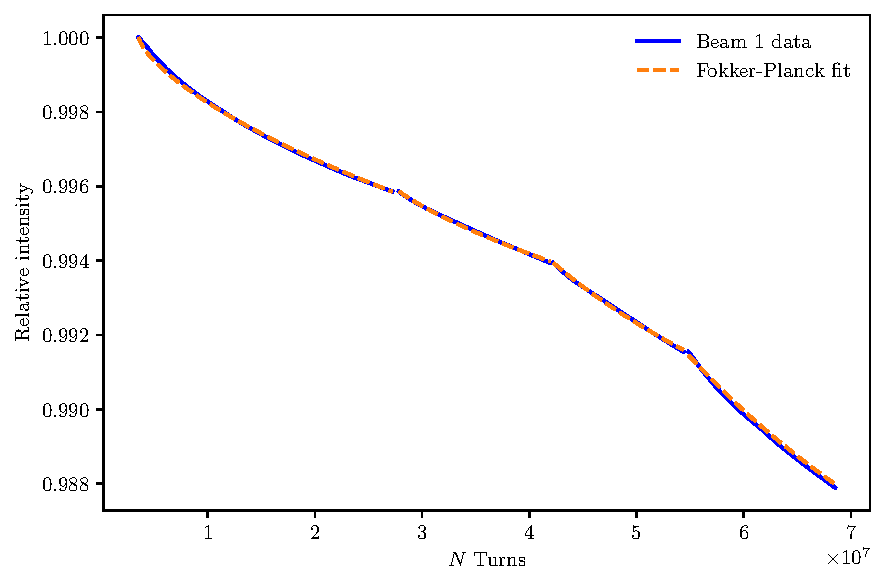
\includegraphics[width=1.0\textwidth]{5_wire_compensators_LHC/figs/losses_b1.pdf}
    \caption{Relative loss of intensity for the data of Beam~1 divided in chunks where the crossing angle is varied. The fit reconstruction is also shown. A good agreement between the data and the fit is observed.}
    \label{fig:reconstruction_1}
\end{figure}

\begin{figure}[hpt]
    \centering
    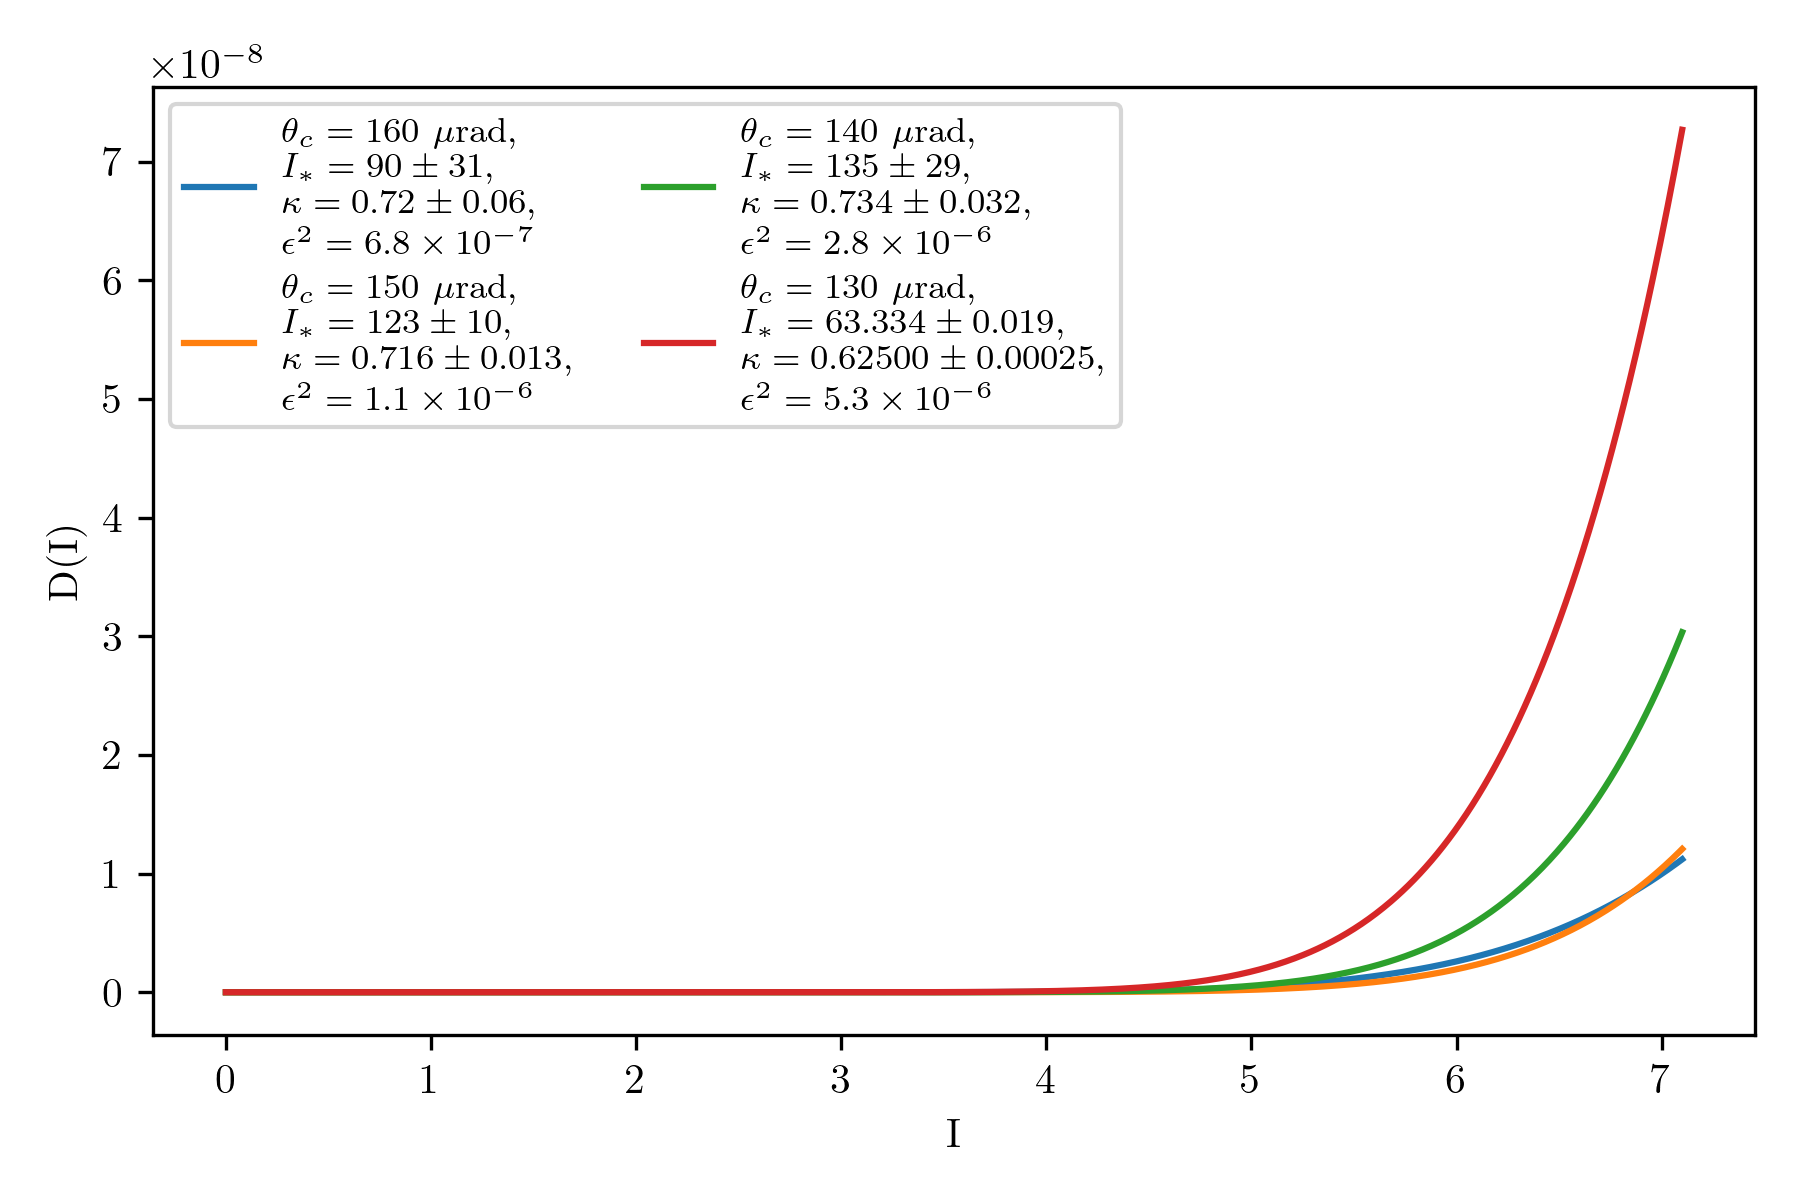
\includegraphics[width=1.0\textwidth]{5_wire_compensators_LHC/figs/fokker_planck_b1_D.png}
    \caption{Reconstructed $D(I)$ for the data of Beam~1 divided in chunks where the crossing angle is varied. The $D(I)$ increases as the crossing angle is lowered.}
    \label{fig:reconstruction_2}
\end{figure}

%\begin{figure}[hpt]
%    \centering
    % \includegraphics[]{}
%    \caption{Evolution of the three parameters, $\epsilon$, $I_\ast$, and $\kappa$, for the data of Beam~1 divided in chunks where the crossing angle is varied. No significant patterns can be observed in the evolution of the parameters.}
%    \label{fig:parameters_1}
%\end{figure}

If instead we consider the data of Beam~1 divided in chunks where the wire compensators are switched on and off, we can see how the $D(I)$ reconstructed, presented in Fig.~\ref{fig:reconstruction_3}, while manifesting differences, does not show a consistent different diffusion value between the two states. Moreover, extreme differences are also obtained from the $D(I)$ reconstructed from the entire chunk also at lower $I$ values. This suggests that the fitting procedure might be affected by overfitting when the chunks are too small and not rich enough in information.

A comparison of the $\chi^2$ values of the fit for the two different slicing methods is shown in Fig.~\ref{fig:chi2}. We can see that the $\chi^2$ values are mostly lower when smaller fragments are considered, but not consistently. This suggests that, since no consistent differences can be observed in the reconstructed $D(I)$ between the wire-on and wire-off states, and as overfitting issues are observed at some fitting chunks, that, indeed, the BBCW on Beam~2 is not significantly affecting the beam dynamics on Beam~1.

\begin{figure}[hpt]
    \centering
    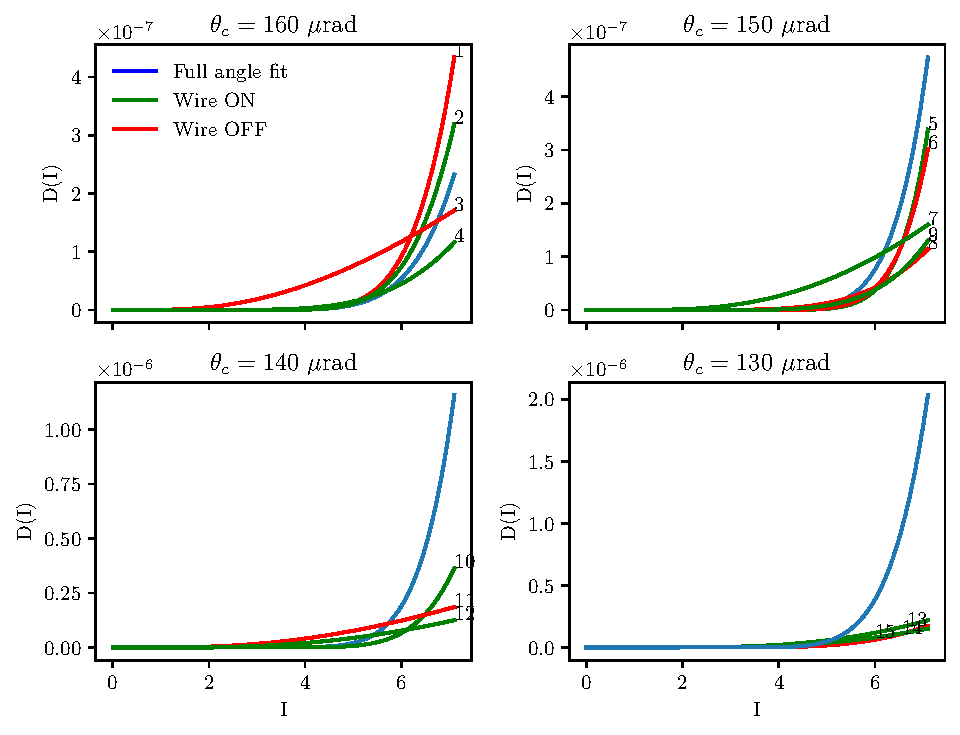
\includegraphics[width=1.0\textwidth]{5_wire_compensators_LHC/figs/fokker_planck_b1_turbo_bis.pdf}
    \caption{Reconstructed $D(I)$ for the data of Beam~1 divided in chunks where the wire compensators are switched on and off, compared with the $D(I)$ reconstructed using the full chunk corresponding to the crossing angle. The $D(I)$ does not show a consistent different diffusion value between the two states and, in multiple situations, the values obtained for $D(I)$ on the smaller samples obtain extremely different results from the full fitting result for low values of $I$. This suggests overfitting issues. The numbers follow the nomenclature in Fig.~\ref{fig:chunks}.}
    \label{fig:reconstruction_3}
\end{figure}

\begin{figure}[hpt]
    \centering
    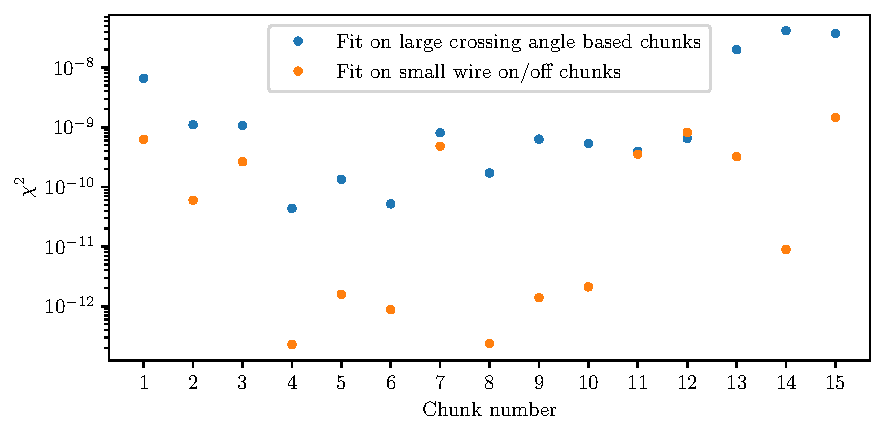
\includegraphics[width=1.0\textwidth]{5_wire_compensators_LHC/figs/chi2_b1.pdf}
    \caption{Comparison of the $\chi^2$ values of the fit for the two different chunking methods. The $\chi^2$ values are mostly lower when smaller chunks are considered, but not consistently so. The numbers follow the nomenclature in Fig.~\ref{fig:chunks}.}
    \label{fig:chi2}
\end{figure}

\subsection*{Beam~2 data}

Now we inspect the data of Beam~2, where the wires are installed. We consider the data divided into chunks as presented in Fig.~\ref{fig:chunks}. In Fig.~\ref{fig:reconstruction_4}, we show the relative intensity loss, along with the fit reconstruction. In Fig.~\ref{fig:reconstruction_5}, we show the reconstructed $D(I)$ for the various crossing angles and the various states of the wire.

It can be seen that, in general, the fit reconstruction is able to reproduce the data quite well. Furthermore, it is possible to see how the reconstructed $D(I)$ is consistently different when the wires are switched on and off, with generally higher diffusion values when the wires are off. This is in agreement with the expectation that the wires are able to reduce the long-range beam-beam effects and thus the diffusion. Moreover, it is possible to see how such a reconstructed $D(I)$ for wire on  also has lower values for low $I$ amplitudes. This suggests that indeed the BBCWs might provide a better long-term stability of the beam.

The values of the two parameters, $I_\ast$ and $\kappa$, are shown in Fig.~\ref{fig:parameters_3}. In addition, in this case, no significant patterns can be observed in the evolution of the parameters for the different states of the system.

%To quantify the effects of the wires on the long-term beam dynamics, we can take the various reconstructed $D(I)$ for one of the crossing angles and consider the evolution of the relative intensity and emittance of a Gaussian distribution with a Fokker-Planck evolution over a number of turns of a higher order of magnitude. In Fig.~\ref{fig:evolution}, we show the evolution of the relative intensity and emittance for the various $D(I)$ reconstructed for the crossing angle of \SI{150}{\micro\radian}. We can see how the wires are able to archive a lower relative intensity. The emittance appear to decrease faster for cases where $D(I)$ is higher, this is due to the functional shape of $D(I)$ that, we recall, implies a semi-stationary distribution following Eq.~\eqref{}, which can be seen in Fig.~\ref{}. Such distribution describes a slow erosion that implies a reduction in emittance.

\begin{figure}[hpt]
    \centering
    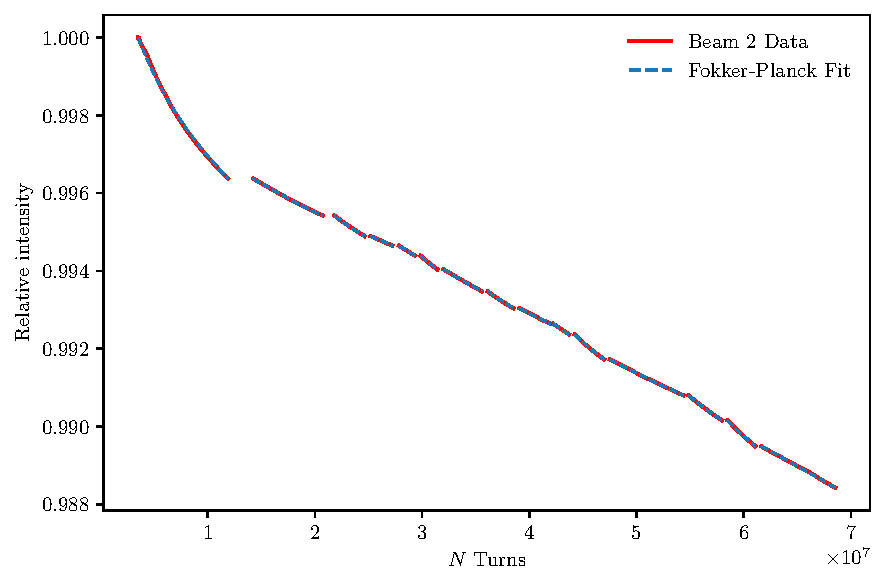
\includegraphics[width=1.0\textwidth]{5_wire_compensators_LHC/figs/losses_b2.pdf}
    \caption{Relative intensity loss and fit reconstruction for the data of Beam~2 divided in chunks, following the nomenclature of Fig.~\ref{fig:chunks}. 
    The fit reconstruction is able to reproduce the data quite well.}
    \label{fig:reconstruction_4}
\end{figure}

\begin{figure}[hpt]
    \centering
    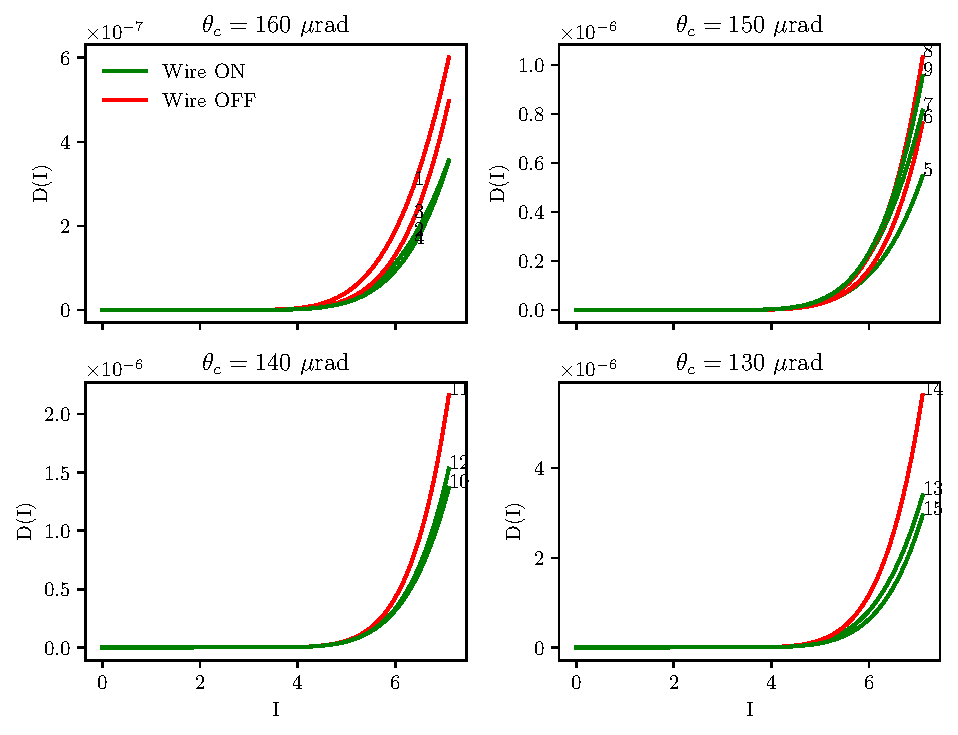
\includegraphics[width=1.0\textwidth]{5_wire_compensators_LHC/figs/fokker_planck_b2_2.pdf}
    \caption{Reconstructed $D(I)$ for the data of Beam~2 divided in chunks, following the nomenclature of Fig.~\ref{fig:chunks}. It can be seen how the reconstructed $D(I)$ is consistently different when the wires are switched on and off, with, in general higher diffusion values when the wires are off. The only exception is given by chunk 6, with a crossing angle of $\theta_c=$\SI{150}{\micro\radian}.}
    \label{fig:reconstruction_5}
\end{figure}

\begin{figure}[hpt]
    \centering
    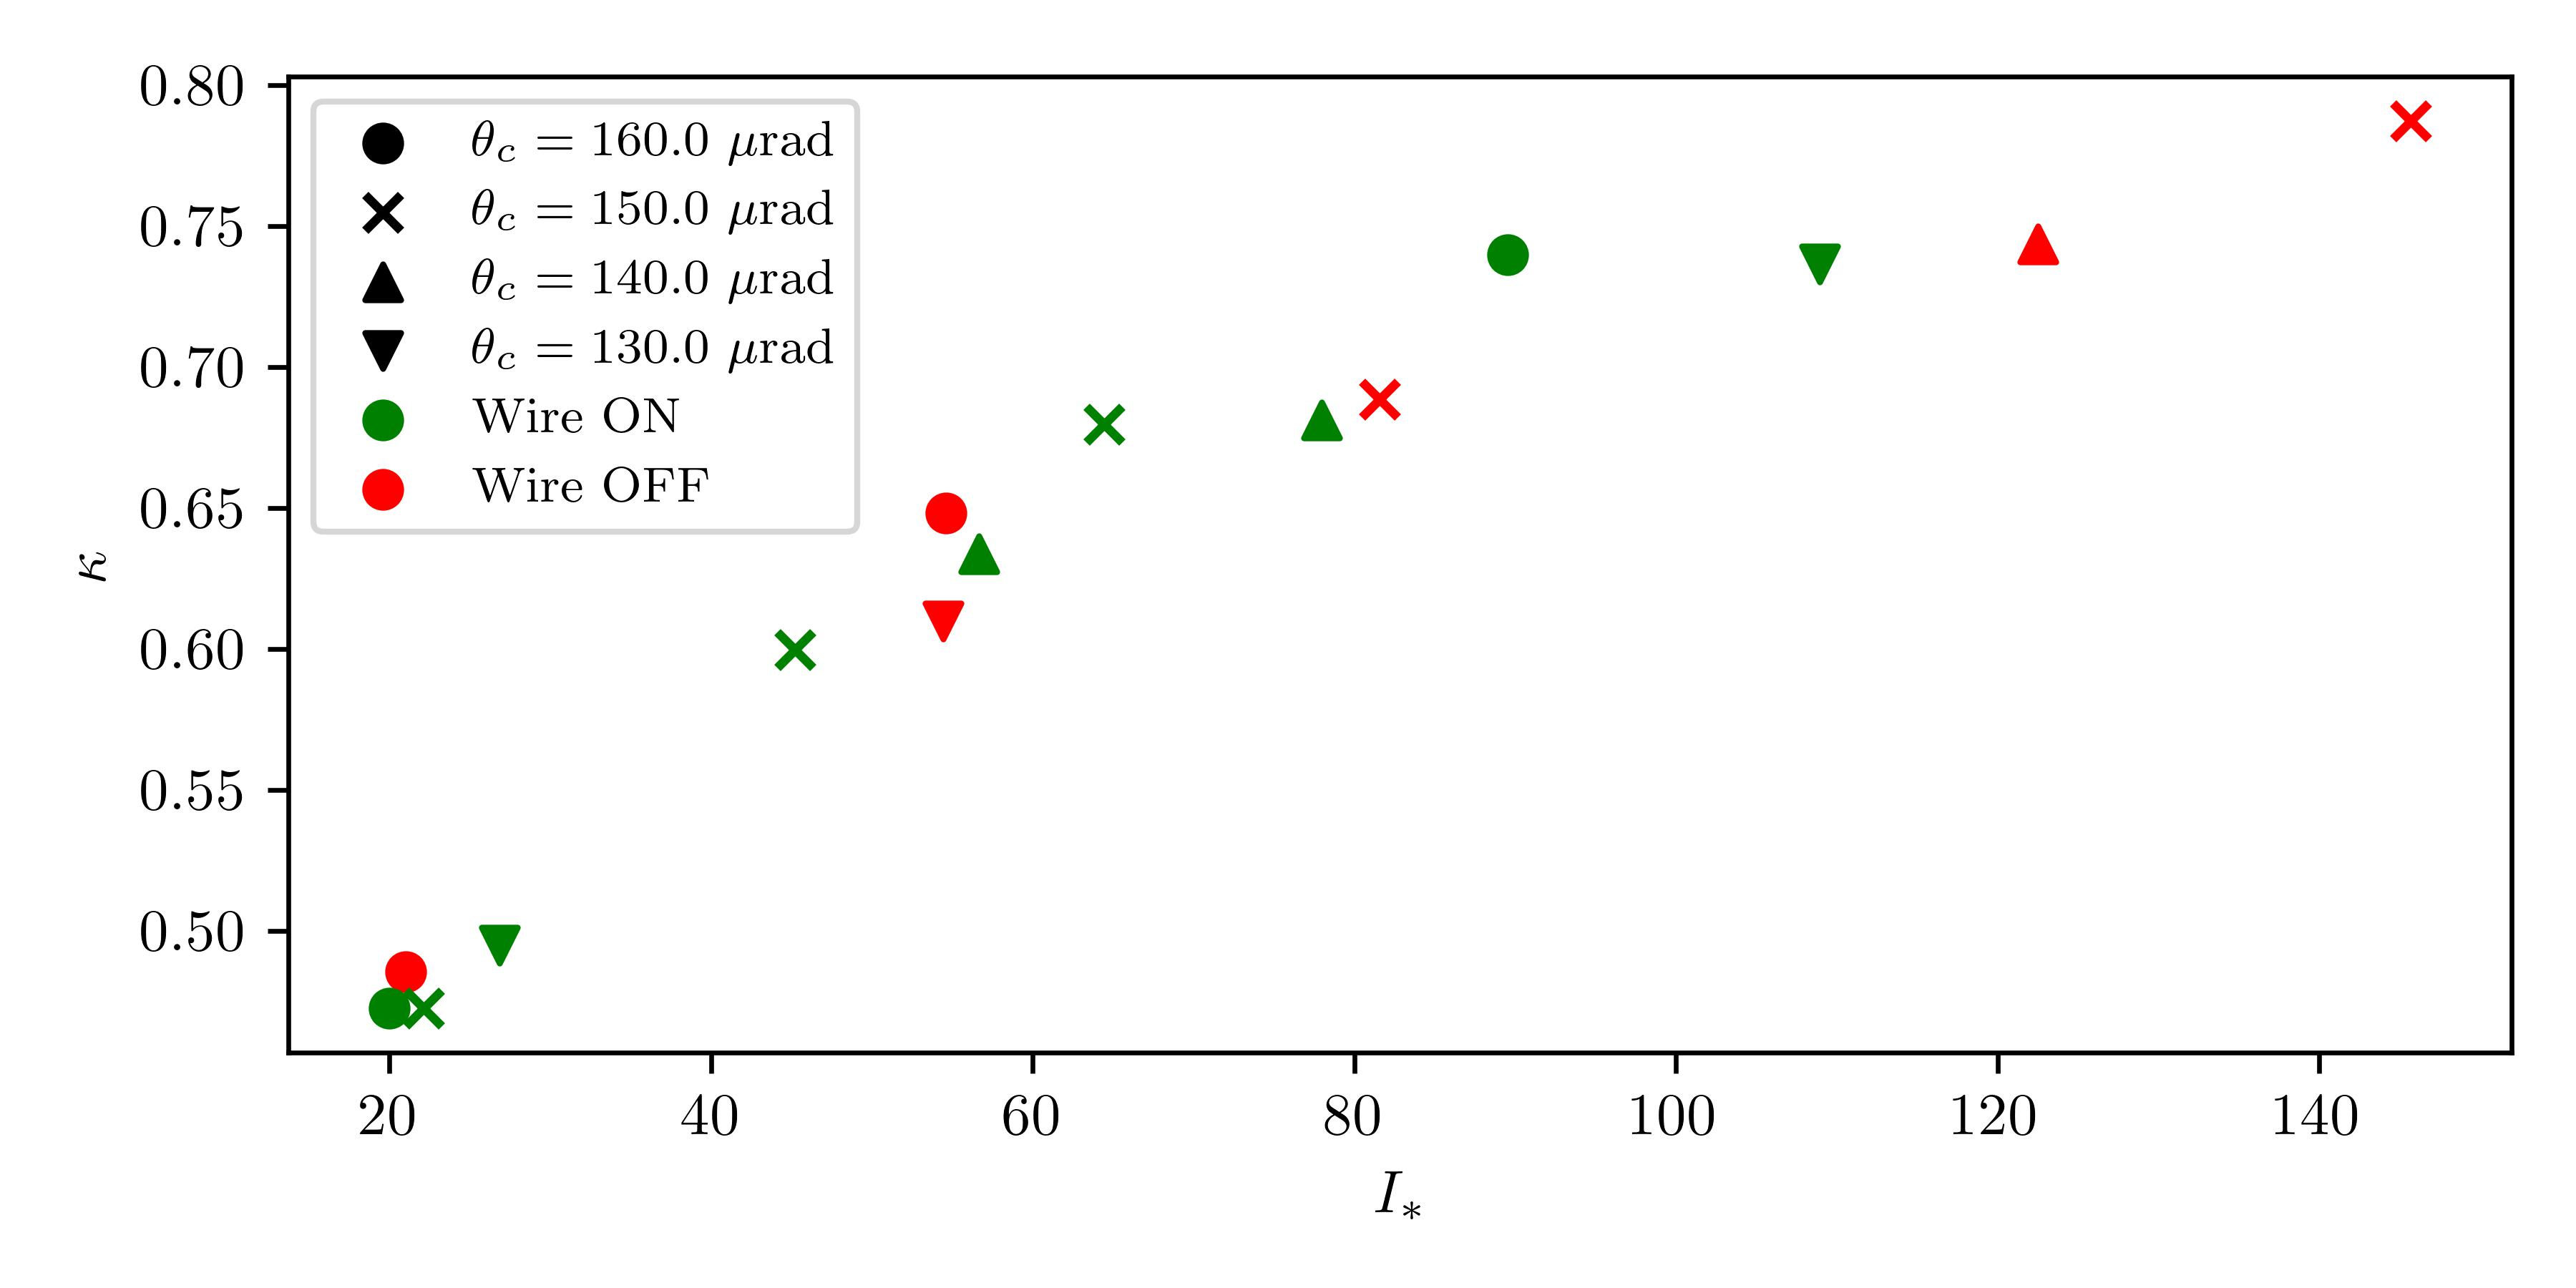
\includegraphics[width=1.0\textwidth]{5_wire_compensators_LHC/figs/fokker_planck_b2.jpg}
    \caption{Evolution of the parameters $I_\ast$, and $\kappa$, for the data of Beam~2 divided in chunks, following the nomenclature of Fig.~\ref{fig:chunks}. No significant patterns can be observed in the evolution of the parameters.}
    \label{fig:parameters_3}
\end{figure}

%\begin{figure}[hpt]
%    \centering
%    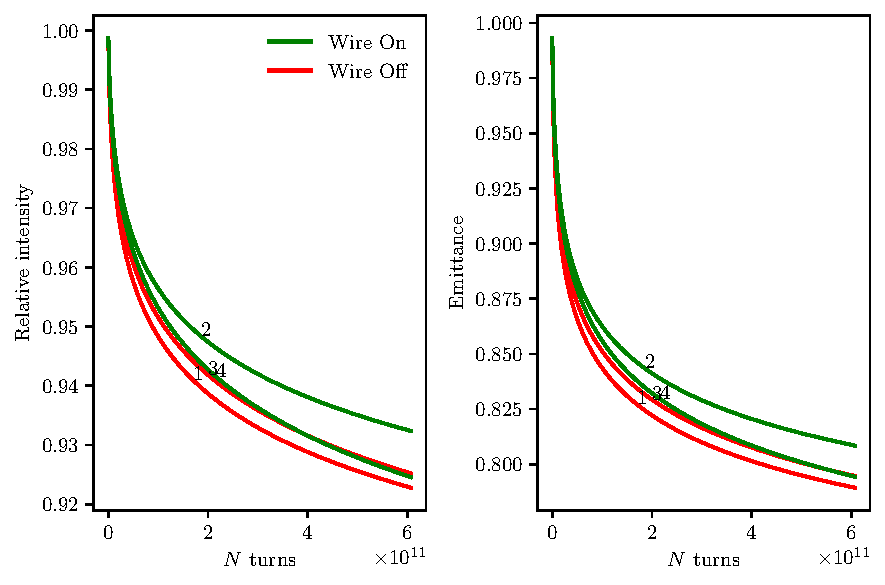
\includegraphics[width=1.0\textwidth]{5_wire_compensators_LHC/figs/sim_emittance.pdf}
%    \caption{Evolution of the relative intensity and emittance for the various $D(I)$ reconstructed for the crossing angle of \SI{160}{\micro\radian}. The evolution is obtained by simulating a Fokker-Planck process, with a Gaussian distribution as initial condition. A lower $D(I)$ yields lower relative losses and lower emittance decrease.}
%    \label{fig:evolution}
%\end{figure}

\section{Final remarks}\label{sec:5:conclusions}

We have performed an initial study of the effects of the BBCWs on the long-term beam dynamics of the LHC using our diffusive framework. We have used the data of the LHC Beam~1 and Beam~2, collected during an MD measurement campaign of Run~2, and we have reconstructed the diffusion coefficient of various system configurations. Ultimately, we have found that the wires are able to reduce the long-range beam-beam effects and thus the diffusion. Moreover, we have observed that our model suggests that the wires are consistently able to reduce the intensity loss. As expected, the model did not highlight significant BBCWs effects on Beam~1.

As pointed out in the overview of the experimental data, a large portion of the data had to be discarded because of the large amount of losses occurring during transient periods. Moreover, multiple chunks considered in the analysis are characterised by a very short time span, which might be too short to be representative of long-term beam dynamics. This is a limitation of the collected data that could have had a significant impact on the results.

However, the promising results obtained in the fit reconstruction seem to suggest that this diffusive framework may provide some insight into the long-term effects of BBCWs on beam dynamics. This has motivated us to consider a different data collection strategy for the scheduled MD measurements of LHC Run~3. More specifically, we planned to measure the BLM losses while keeping the BBCWs on and off for longer time spans, to better characterise the long-term effects of the wires.

Additionally, we planned to perform collimation scans with BBCWs on and off, in order to directly inspect the beam tail population and measure $D(I)$ following the protocol presented in Chapter~\ref{ch:probing}. The purpose was to compare the values obtained with the two different methodologies.

Both of these strategies in the data gathering have been successfully implemented during a MD measurement campaign of LHC Run3~\cite{}, and the results will be presented in a future work.